%! Licence = CC BY-NC-SA 4.0

%! Author = gianfluetsch
%! Date = 22. Jan 2022
%! Project = icth_summary

\section{Kanalcodierung}

\subsection{Blockcode}
\subsubsection{Nachprüfung HS2020}
$x_5=x_1+x_2+x_3$\\
$x_6=x_1+x_2+x_4$\\
$x_7=x_2+x_3+x_4$

\paragraph{Prüfmatrix des Blockcodes}\mbox{}\\
$\begin{matrix}
    x_1 & x_2 & x_3 & x_4 & | & x_5 & x_6 & x_7\\
    1 & 1 & 1 & 0 & | & 1 & 0 & 0\\
    1 & 1 & 0 & 1 & | & 0 & 1 & 0\\
    0 & 1 & 1 & 1 & | & 0 & 0 & 1
\end{matrix}$

\paragraph{Anzahl Kontrollstellen}\mbox{}\\
Anzahl Kontrollstellen = Anzahl 1 in Prüfmatrix (Einheitsmatrix) $\rightarrow$ 3

\paragraph{Anzahl gültige Codeworte mit Blockcode}\mbox{}\\
gültige Codeworte = Anzahl Spalten ohne Prüfmatrix\\
$m=4 \rightarrow 2^m=2^4=16$

\paragraph{Fehlersyndom, falls x1 und x2 gestört}\mbox{}\\
$110$\\
$111$\\
$--$\\
$001$

\paragraph{Fehler erkennen}\mbox{}\\
Ja, der Fehler (Syndrom) liegt in der Spalte $x_7$ der Prüfmatrix.
Geht man nun davon aus, dass nur ein Fehler passiert ist, so wird man hier eine Falschkorrektur vornehmen
(durch flippen des siebten Bits)

\paragraph{Fehler korrigieren?}\mbox{}\\
Nein, Fehler kann nicht korrigiert werden, da er in der regulären Prüfmatrix nicht gefunden wurde.

\subsubsection{Prüfung Fs2017}
Gegeben ist die folgende Generatormatrix eines systematischen Blockcodes mit den Prüfvektoren $p_1$ bis $p_7$:
$\begin{matrix}
    p_1 & p_2 & p_3 & p_4 & p_5 & p_6 & p_7\\
    1 & 0 & 1 & 1 & 0 & 0 & 0\\
    1 & 1 & 1 & 0 & 1 & 0 & 0\\
    1 & 1 & 0 & 0 & 0 & 1 & 0\\
    0 & 1 & 1 & 0 & 0 & 0 & 1
\end{matrix}$

\paragraph{Wie viele Nachrichtenstellen m hat der Code?}\mbox{}\\
Code hat 3 Nachrichtenstellen

\paragraph{Wie viele Kontrollstellen k hat der Code?}\mbox{}\\
Der Code hat 4 Kontrollstellen

\paragraph{Wie lautet das Fehlersyndrom, wenn nur das dritte Bit einer Nachricht falsch übertragen wird?}\mbox{}\\
101

\paragraph{Ermitteln Sie die Hamming-Distanz des Codes}\mbox{}\\
$H=4$\\
Es müssen mindestens 4 Prüfvektoren addiert werden, um den Orginalen-Vektor zu erhalten.

\paragraph{Ist der Code dicht gepackt?}\mbox{}\\
Der Code ist nicht dichtgepackt, da $H=4$ ist. Damit liegt mindestens 1 Codewort (CW) ausserhalb \textit{einer Korrigierkugel}.

\subsubsection{Prüfung FS2015}
Gegeben ist die folgende Prüfmatrix eines  Hamming Blockcode
\begin{center}
    \vspace{-8pt}
    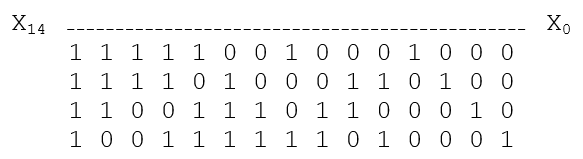
\includegraphics[width=.7\linewidth]{./02-kanalcodierung/fs2015_1}
    \vspace{-8pt}
\end{center}

Wie gross ist die
\begin{itemize}
    \item Anzahl der Kontrollstellen: $k=4$
    \item Anzahl Nachrichtenstellen: $m=2^4-1-k=11$
    \item Codewortlänge CW: $2^4-1=15$
    \item Anzahl korrigierbare Fehler: $1$
    \item Anzahl gültige Codeworte: $2^11=2048$\\
\end{itemize}

Bestimmen sie für den Fall, dass die Codestellen x13 und x11 fehlerhaft sind das Fehlersyndrom?\\
Syndrom $(0011)^T$\\

Was würde bei einer Vorwärtskorrektur passieren?\\
\textit{x6 würde fälschlicherweise Korrigiert.}

\subsubsection{Prüfung HS2009}
Gegeben sind die folgenden Fehlersyndrome für einen einzigen Bitfehler an der jeweiligen Stelle xi eines systematischen Blockkodes:\\
$Z(x1)=[111], Z(x2)=[110], Z(x3)=[101], Z(x4)=[011], Z(x5)=[100], Z(x6)=[010], Z(x6)=[001]$\\

Geben Sie die Generatormatrix des Blockcodes an.\\
$\begin{matrix}
    x1 & x2 & x3 & x4 & x5 & x6 & x7\\
    1 & 1 & 1 & 0 & 1 & 0 & 0\\
    1 & 1 & 0 & 1 & 0 & 1 & 0\\
    1 & 0 & 1 & 1 & 0 & 0 & 1
\end{matrix}$

Wie gross ist die Hammingdistanz des Codes?\\
$h=3$\\
% TODO: Hamming-Distanz = Anzahl Kontrollstellen?

Ermittelten sie für die unten aufgeführten Nachrichtenwörter die vollständigen Codewörter\\
$NW1 = x6 = 0001$ $\textcolor{red}{0}$ $\textcolor{red}{1}$ $\textcolor{red}{1}$\\
$NW2 = x7 = 1010$ $\textcolor{red}{0}$ $\textcolor{red}{1}$ $\textcolor{red}{0}$

\subsubsection{Prüfung FS2009}
Gegeben ist die folgende Generatormatrix.
\begin{center}
    \vspace{-8pt}
    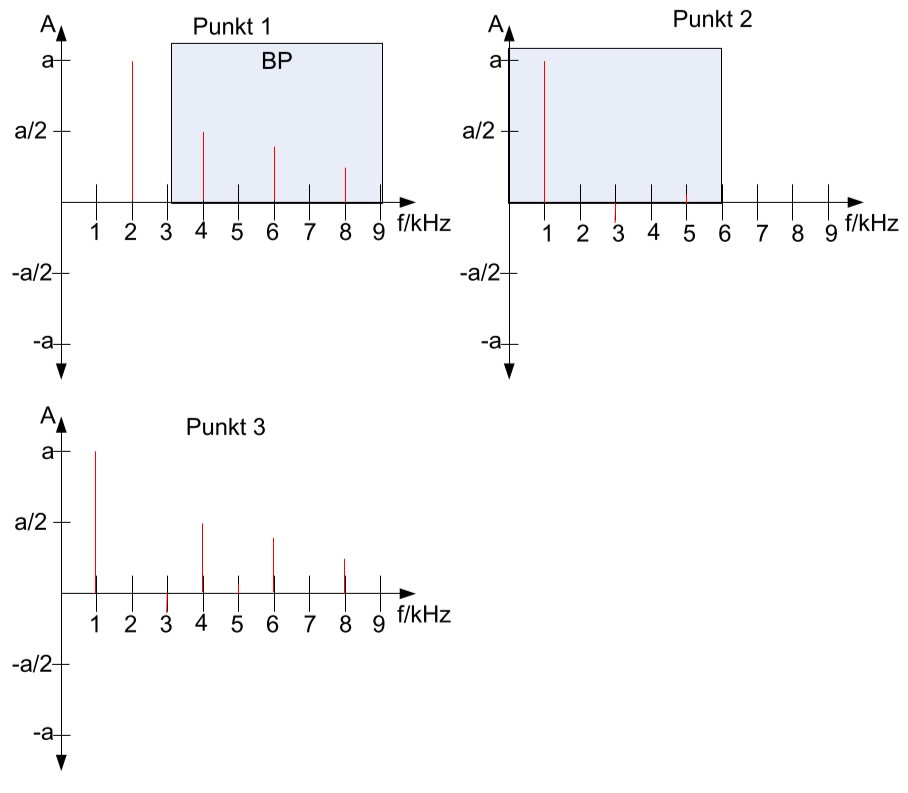
\includegraphics[width=.8\linewidth]{./02-kanalcodierung/fs2009_2}
    \vspace{-8pt}
\end{center}

Wie gross ist die Anzahl der Kontrollstellen k und der Nachrichtenstellen m?\\
$k=4, m=11$\\

Sie empfangen die folgenden Codewörter.
\begin{center}
    \vspace{-8pt}
    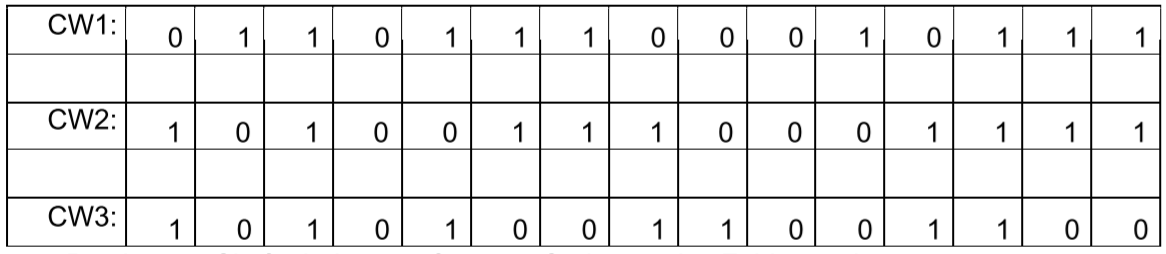
\includegraphics[width=.8\linewidth]{./02-kanalcodierung/fs2009_3}
    \vspace{-8pt}
\end{center}

\begin{itemize}
    \item Bestimmen Sie für jedes empfangene Codewort das Fehlersyndrom.
    \item Bestimmen sie ferner, welche Codewörter wahrscheinlich korrekt und welche fehlerhaft übertragen wurden.
    \item Im Fehlerfall geben Sie bitte an, welche Stelle voraussichtlich gestört wurde.
\end{itemize}
\textit{CW1: 1 1 0 1, Fehlerposition: x6}\\
\textit{CW2: 1 0 1 0, Fehlerposition: x4}\\
\textit{CW3: kein Fehler!}\\

Konstruieren Sie einen (reduzierten) Hamming-Code (Generatormatrix) für den Fall, dass Sie 8-stellige Nachrichten gegen Übertragungsfehler absichern müssen. Warum spricht man von einem reduzierten Code?\\
\begin{center}
    \vspace{-8pt}
    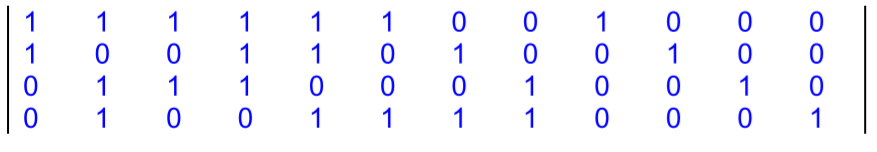
\includegraphics[width=.8\linewidth]{./02-kanalcodierung/fs2009_4}
    \vspace{-8pt}
\end{center}
\textit{Reduzierter Code: Weil die Anzahl der Nachrichtenstellen nicht vollständig ausgenutzt werden.}

\subsection{Zyklischer Code}
\subsubsection{Nachprüfung HS2020}
Gegeben ist folgendes Generatorpolynom:
$p(x)=x^5+x^3+x^2+1$

\paragraph{Wie viele Kontrollstellen hat Code}\mbox{}\\
Grad 5 $\rightarrow$ 5 Kontrollstellen

\paragraph{Schieberegister}\mbox{}\\
\begin{center}
    \vspace{-8pt}
    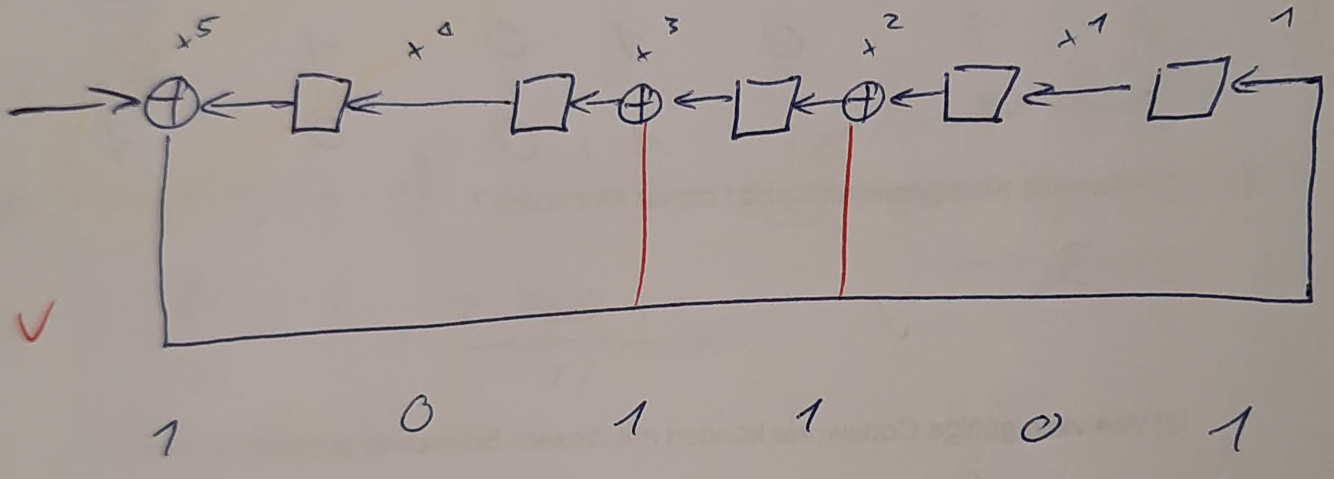
\includegraphics[width=.8\linewidth]{./02-kanalcodierung/schieberegister}
    \vspace{-8pt}
\end{center}

\paragraph{Prüfen, ob Codewort gültig}\mbox{}\\
Prüfmatrix aus Schieberegister ablesen (101101).
\begin{center}
    \vspace{-8pt}
    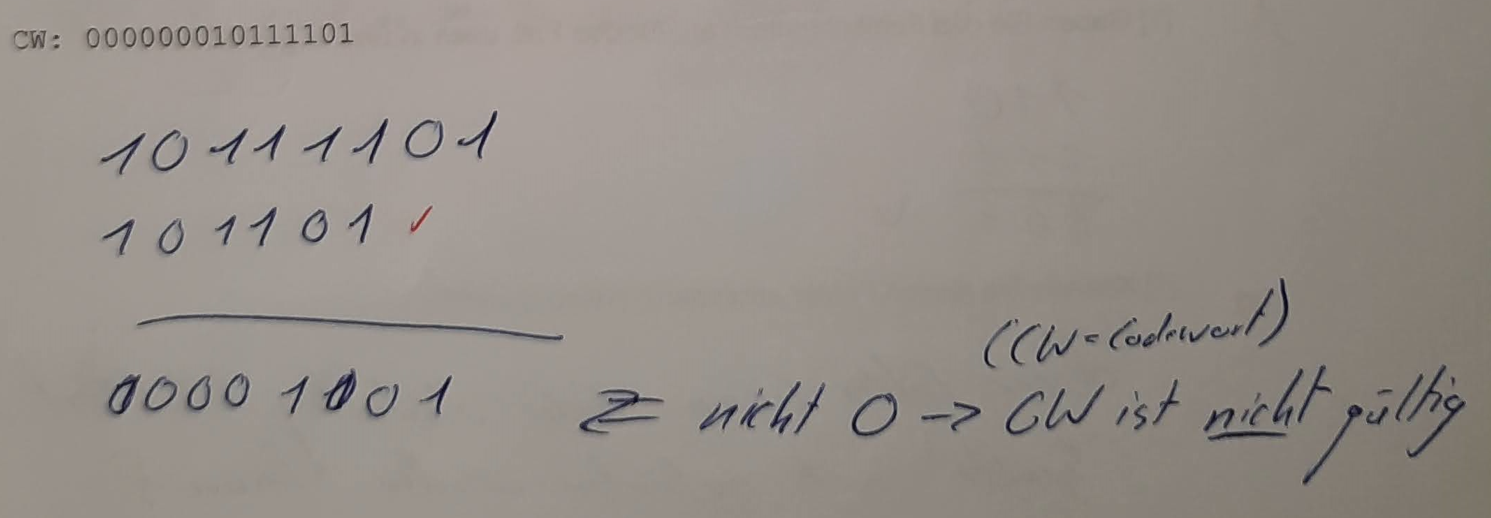
\includegraphics[width=.8\linewidth]{./02-kanalcodierung/codewort}
    \vspace{-8pt}
\end{center}

\paragraph{Fehlersyndrom für Stelle $x^5$ mit Polynomdivison ermitteln}\mbox{}\\
$x^5:x^3+x^2+1 \rightarrow Rest: x+1$

\subsubsection{Prüfung FS2017}
Gegeben ist das folgende Generatorpolynom:\\
$g(x)=x^4+x^3+x^2+1$

\paragraph{Ist das Generatorpolynom irreduzibel?}\mbox{}\\
\begin{center}
    \vspace{-8pt}
    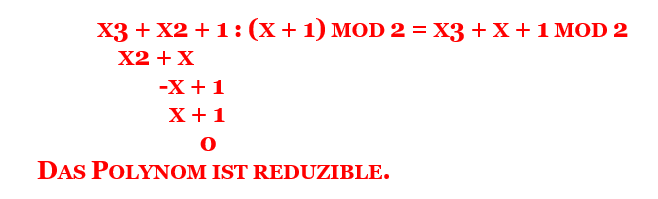
\includegraphics[width=.8\linewidth]{./02-kanalcodierung/fs2017}
    \vspace{-8pt}
\end{center}

\paragraph{Ermitteln Sie die Kontrollstellen für die Nachricht m=100}\mbox{}\\
\begin{center}
    \vspace{-8pt}
    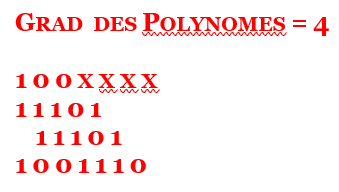
\includegraphics[width=.5\linewidth]{./02-kanalcodierung/fs2017_1}
    \vspace{-8pt}
\end{center}

\paragraph{Ermitteln Sie die Zyklusfolge des Polynoms}\mbox{}\\
$A4+A3+A2=1$\\
$0,(1=A0),A,A2,A3$\\

$A4=A3+A2+1$\\

$A5 = A4 + A3 + A = A3 + A2 + 1 +  A3 + A =  A2 + A + 1$\\
$A6= A3 + A2 + A$\\
$A7= A4 + A3 + A2 = A3 + A2 + 1 + A3 + A2 = 1$\\
Somit ergibt sich der Zyklus zu: 0001, 0010, 0100, 1000, 1101, 1110, 0001

\subsubsection{Prüfung FS2015}
Gegeben ist das folgende Generatorpolynom p:\\
$p(x)=1+x^2+x^6+x^{10}+x^{14}$\\

Prüfen Sie durch Rechnung, ob das Polynom irreduzibel ist.
\begin{center}
    \vspace{-8pt}
    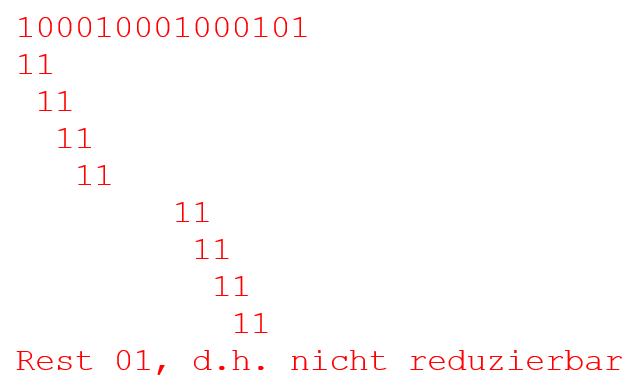
\includegraphics[width=.5\linewidth]{./02-kanalcodierung/fs2015_2}
    \vspace{-8pt}
\end{center}

Wie gross sind in diesem Fall
\begin{itemize}
    \item Kontrollstellenzahl (k): $k=14$
    \item Nachrichtenzahl (m): $m=2^{14}-1-14=16369$
    \item Codewortlänge (n): $n=2^{14}-1=16383$
\end{itemize}

\subsubsection{Prüfung HS2009}
Gegeben ist das folgende Generatorpolynome p\\
$p(x)=1+x^2+x^4+x^5$\\

Wie gross ist die Anzahl der Nachrichtenstellen m, die Kontrollstellen k sowie die Hammingdistanz h? (Achtung: Ist das Polynom prim?)\\
Das Polynom ist nicht prim:\\
$(x^5+x^4+x^2+1):(x+1)=(x^4+x+1)(x+1)$\\
d.h. $h=4,k=5,n=2^4-1=15 \rightarrow m=10$\\

Prüfen sie, ob das Generatorpolynom $p_1(x)=1+x+x^4+x^5$ das folgende Codewort gültig ist.\\
\begin{center}
    \vspace{-8pt}
    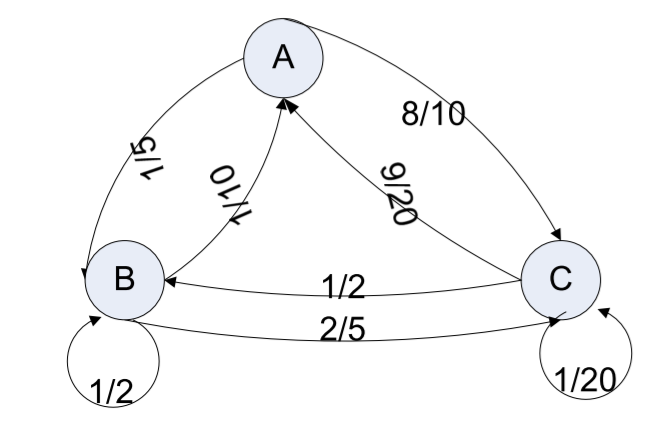
\includegraphics[width=.5\linewidth]{./02-kanalcodierung/hs2009_2}
    \vspace{-8pt}
\end{center}

\subsubsection{Prüfung FS2009}
Gegeben sind die folgenden Generatorpolynome p1 und p2:\\
$p_1(x)=1+x+x4$\\
$p_2(x)=1+x2+x4+x5$\\

Zeigen Sie, dass ein Generatorpolynom einen Hamming-Code und das andere einen Abramson-Code darstellt.\\
\textit{Hamming-Code: p1 nicht weiter teilbar}\\
\textit{Abramson-Code: p2, p1*(1+x)}\\

Wie gross ist jeweils die Anzahl der Nachrichtenstellen m, die Kontrollstellen k sowie die Hammingdistanz h?\\
$p_1: k=4, m=11, h=3$\\
$p_2: k=5, m=10, h=4$\\

Geben Sie für das Generatorpolynom p1(x)=1+x+x4 das rückgekoppelte Schieberegister zur Ermittlung der Kontrollstellen an.
\begin{center}
    \vspace{-8pt}
    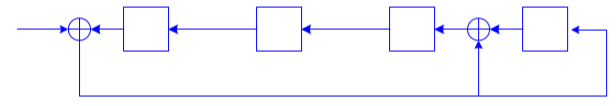
\includegraphics[width=.7\linewidth]{./02-kanalcodierung/fs2009_5}
    \vspace{-8pt}
\end{center}

Geben Sie mit Hilfe des Schieberegisters an, ob das folgende Codewort gültig ist (Weg muss ersichtlich sein). CW: 000 0000 1011 1101
\begin{center}
    \vspace{-8pt}
    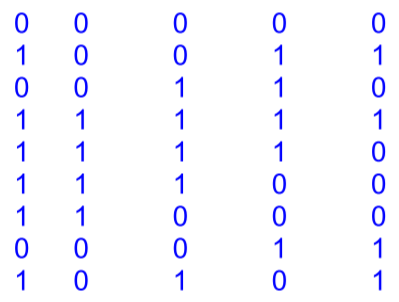
\includegraphics[width=.3\linewidth]{./02-kanalcodierung/fs2009_6}
    \vspace{-8pt}
\end{center}

\subsection{Faltungscode}
\subsubsection{Nachprüfung HS2020}\mbox{}\\
\begin{center}
    \vspace{-8pt}
    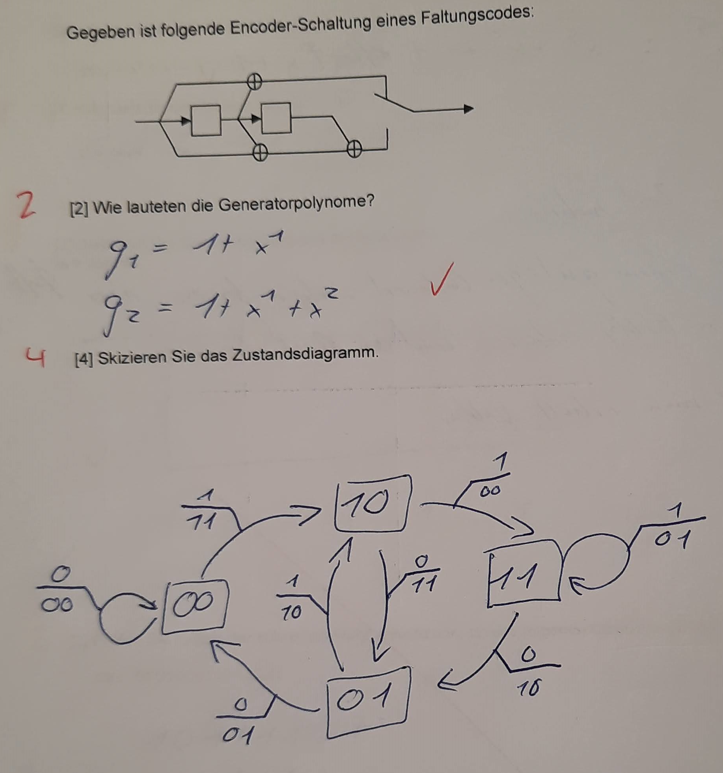
\includegraphics[width=.8\linewidth]{./02-kanalcodierung/faltungscode}
    \vspace{-8pt}
\end{center}

\subsubsection{Prüfung FS2017}
Gegeben ist der folgende Faltungscodierer
\begin{center}
    \vspace{-8pt}
    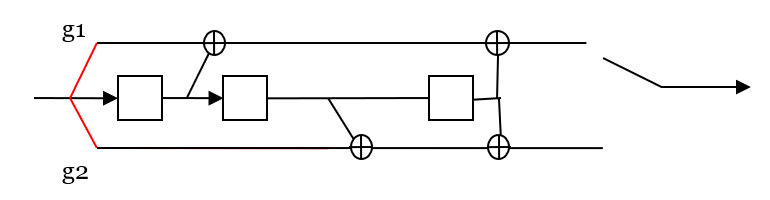
\includegraphics[width=.8\linewidth]{./02-kanalcodierung/fs2017_2}
    \vspace{-8pt}
\end{center}

\paragraph{Wie viele Bits werden zur Berechnung der Ausgangsbit herangezogen?}\mbox{}\\
4, drei aus dem Speicher und das aktuelle


\paragraph{Bestimmen Sie die Impulsantwort der Decoderschaltung}\mbox{}\\
\begin{center}
    \vspace{-8pt}
    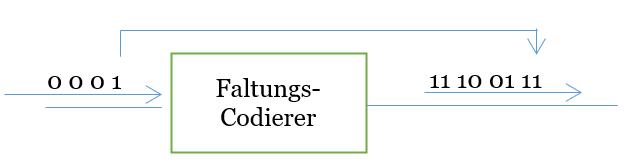
\includegraphics[width=.8\linewidth]{./02-kanalcodierung/fs2017_3}
    \vspace{-8pt}
\end{center}

\paragraph{Geben Sie die Codes in Polynomdarstellung an}\mbox{}\\
$g_1=x^3+x+1$\\
$g_2=x^3+x^2+1$

\paragraph{Wie viele Zustände hat der Coder?}\mbox{}\\
8

\paragraph{Bestimmen Sie seine Coderate}\mbox{}\\
$\frac{Anzahl Ausgangsbits}{Anzahl Eingangsbits} = \frac{8}{4}=2$\\

\subsubsection{Prüfung HS2016}
Gegeben seien die folgenden Impulsantworten eines (3,1,2)-Faltungscodierers:\\
${g_1}={1,1,0}, {g_2}={1,0,1} \& {g_3}={1,1,1}$\\

\paragraph{Zeichnen Sie die Encoder Schaltung}\mbox{}\\
\begin{center}
    \vspace{-8pt}
    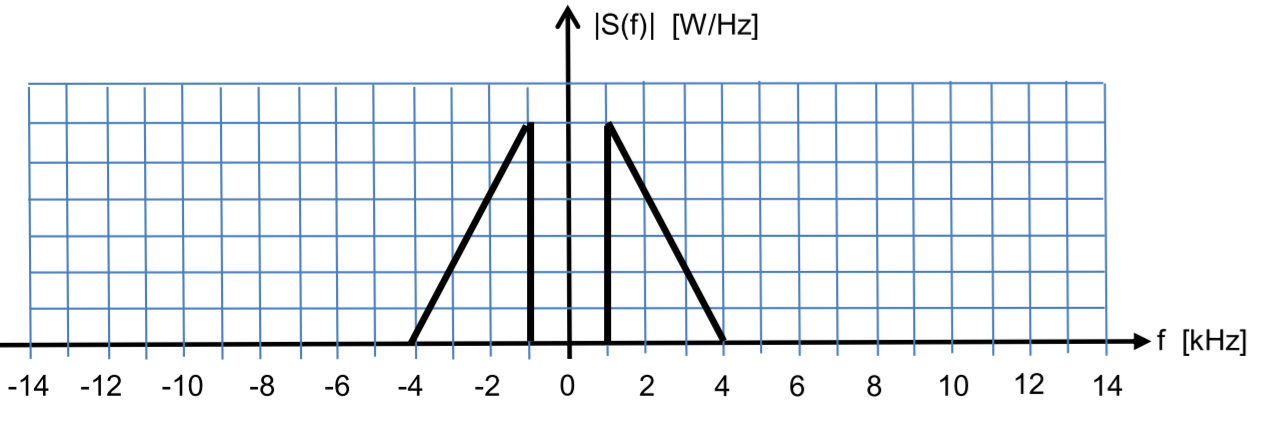
\includegraphics[width=.8\linewidth]{./02-kanalcodierung/hs2016}
    \vspace{-8pt}
\end{center}

\paragraph{Wie viele Tail-Bits müssen einer Nachrichtenfolge angefügt werden?}\mbox{}\\
2 TAIL-BITS

\paragraph{Geben Sie das Encoder-Zustandsdiagramm an}\mbox{}\\
\begin{center}
    \vspace{-8pt}
    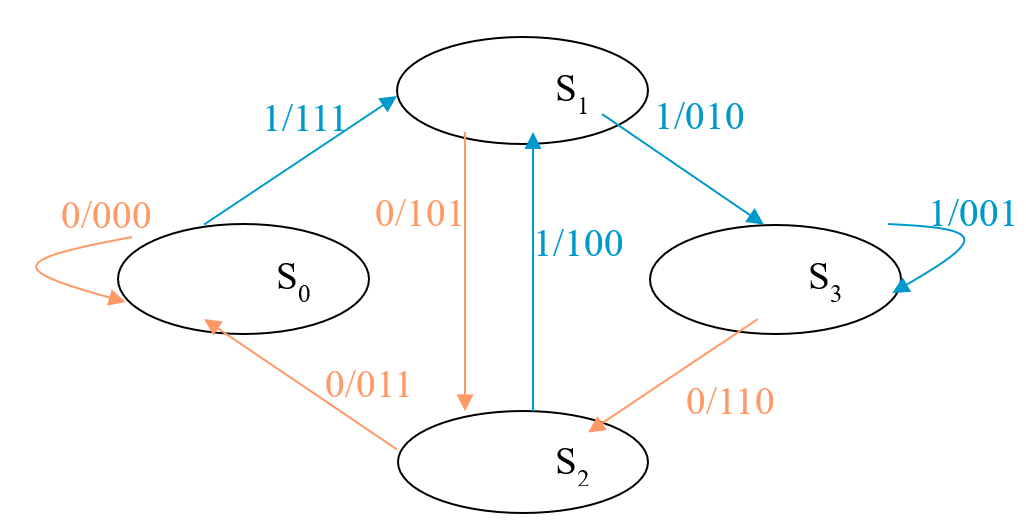
\includegraphics[width=.8\linewidth]{./02-kanalcodierung/hs2016_1}
    \vspace{-8pt}
\end{center}

\paragraph{Liegt ein katastrophaler Code vor (Begründung)?}\mbox{}\\
Nein, da es keine Zyklen ohne Gewichtszunahme gibt.

\paragraph{Bestimmen sie die (Block)-Coderate}\mbox{}\\
$B=Eingabebits$\\
$R=\frac{B}{N} = \frac{B}{3*(B+2)}$

\subsubsection{Prüfung HS2009}
Gegeben seien die folgenden Impulsantworten eines Faltungscodierers mit einem Eingang:\\
${g1}={1,1,0}$ und ${g2}={1,1,1}$\\

Zeichen Sie die Encoder Schaltung.
\begin{center}
    \vspace{-8pt}
    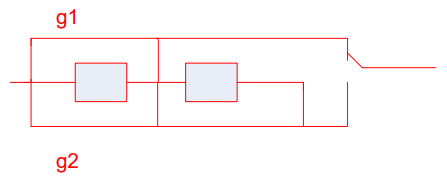
\includegraphics[width=.8\linewidth]{./02-kanalcodierung/hs2009_3}
    \vspace{-8pt}
\end{center}

Wie viele Tail-Bits müssen einer Nachrichtenfolge angefügt werden?\\
\textit{2 Tailbits}\\

Geben Sie das Encoder-Zustandsdiagramm an.\\
\begin{center}
    \vspace{-8pt}
    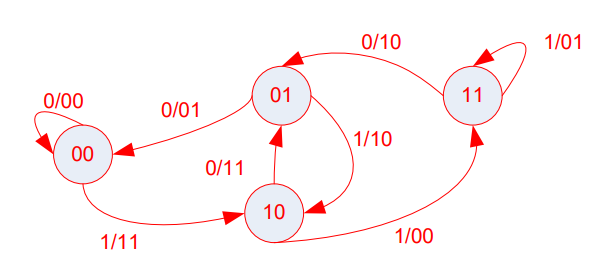
\includegraphics[width=.8\linewidth]{./02-kanalcodierung/hs2009_4}
    \vspace{-8pt}
\end{center}

Handelt es sich um einen „Guten Code“ (Mit Begründung)?\\
\textit{Ja, da der Unterschied der Ausgabe bei einem Zustandsübergang immer maximal ist.}\\

Ermitteln Sie für die Nachrichtenfolge ${u[n]}={1,0,1,1,0,1,1}$ die Ausgangscodefolge {v[n]}.\\
\begin{center}
    \vspace{-8pt}
    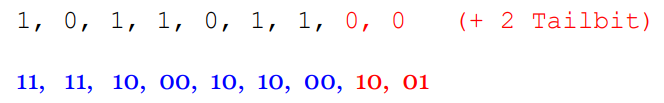
\includegraphics[width=.8\linewidth]{./02-kanalcodierung/hs2009_5}
    \vspace{-8pt}
\end{center}

\subsubsection{Prüfung FS2009}
Gegeben seien die folgenden Impulsantworten eines (2,1,2)-Faltungscodierers: {g1}={1, 1, 0} und {g2}={1, 0, 1}\\

Zeichnen Sie die Encoder-Schaltung.
\begin{center}
    \vspace{-8pt}
    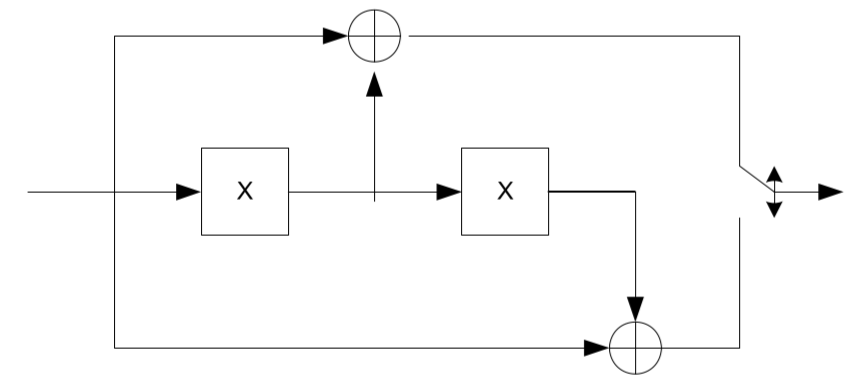
\includegraphics[width=.8\linewidth]{./02-kanalcodierung/fs2009_7}
    \vspace{-8pt}
\end{center}

Wie viele Tail-Bits müssen einer Nachrichtenfolge angefügt werden?\\
\textit{2 Tail-Bits}\\

Geben Sie das Encoder-Zustandsdiagramm an.
\begin{center}
    \vspace{-8pt}
    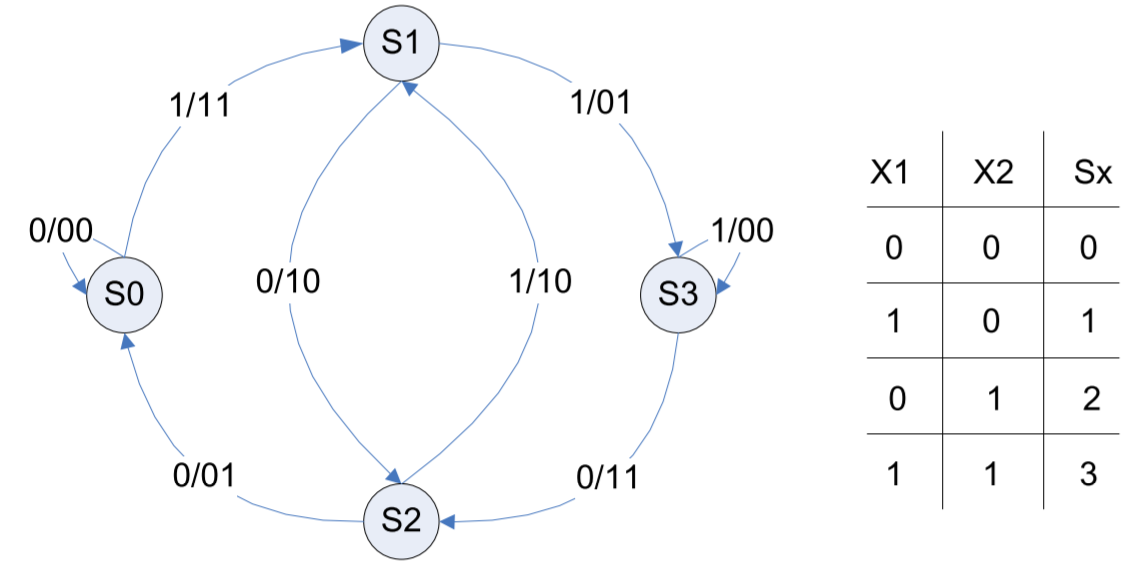
\includegraphics[width=.8\linewidth]{./02-kanalcodierung/fs2009_8}
    \vspace{-8pt}
\end{center}

Lieft ein katastrophaler Code vor?\\
\textit{Ja, da keine Gewichtszunahme beim Zustand S3 wenn eine 1 kommt. 1 Folge geht in eine 0 Folge über.}\\

Ermitteln Sie für die Nachrichtenfolge {u[n]}={1,1,1,0,1,1} die Ausgangscodefolge {v[n]}.\\
${v[n]}={1,1,0,1,0,0,1,1,1,0,0,1,Tailbits,1,1,0,1}$\\

Bestimmen sie für das obige Beispiel die (Block-)Coderate.\\
$R=b/n$\\
$b=Eingabebits=6$\\
$n=Ausgabebits=6*2+2*2 (Tail-Bits)$\\
$R=6/16=0.375$

\subsection{Kanalmatrix}
\subsubsection{Prüfung HS2016}
Die Eigenschaften eines Kanals seien durch die folgende Kanalmatrix beschrieben: 

$P(Y|X) = \begin{matrix}
    0.4 & 0.5 & 0.1\\
    0.3 & 0.4 & 0.3\\
    0.3 & 0.1 & 0.6
\end{matrix}$

\paragraph{Bestimmen Sie die Entscheidungszuordnung nach dem Maximum Likelyhood-Verfahren:}\mbox{}\\
$P(Y|X) = \begin{matrix}
    \textcolor{red}{0.4} & \textcolor{red}{0.5} & 0.1\\
    0.3 & 0.4 & 0.3\\
    0.3 & 0.1 & \textcolor{red}{0.6}
\end{matrix}$

\paragraph{}\mbox{Maximum Likelihood}\\
Berechnen Sie die Restfehlerwahrscheinlichkeit für die nach dem Maximum Li-kelyhood-Verfahren gefundene Entscheidungszuordnung\\
Gehen Sie davon aus, dass alle Eingangszeichen gleichwahrscheinlich auftreten.\\

$p(restfehler) = 1 - [1/3*(0.4+0.5+0.6)] = 0.5$\\

In einer vertieften Analyse der Eingangszeichen wurden folgende Auftrittshäufigkeiten festge-stellt:\\
$x1 = 500$\\
$x2 = 2500$\\
$x3 = 7000$\\

Lässt sich mit dieser zusätzlichen Information eine Entscheidungszuordnung finden, die besser ist als die nach dem Maximum Likelyhood-Verfahren gefunde-ne? Begründen Sie Ihren Entscheid.
$p(x1) = 0.05$\\
$p(x2) = 0.25$\\
$p(x3) = 0.70$\\


$P(Y|X) = \begin{matrix}
    \textcolor{red}{0.4} & 0.5 & 0.1\\
    0.3 & \textcolor{red}{0.4} & 0.3\\
    0.3 & 0.1 & \textcolor{red}{0.6}
\end{matrix}$

$p(rest) = 1-(0.05*0.4 + 0.25*0.4 + 0.7*0.6) = 0.46 $\\

ist kleiner als 0.5 und auch kleiner als wenn Restfehlerwahrscheinlichkeit mit der Analyse für 	die ursprünglich gewählte Konfiguration:\\
$1 - (0.05*0.4 + 0.05*0.5 + 0.7*0.6) = 0.535$

\subsection{Kanal}
\subsubsection{Prüfung FS2015}
Messungen an einem symmetrischen Kanal, ergeben die unten angegebenen Auftrittswahrscheinlichkeiten der Zeichen am Kanaleingang respektive am Kanalausgang.\\
\begin{center}
    \vspace{-8pt}
    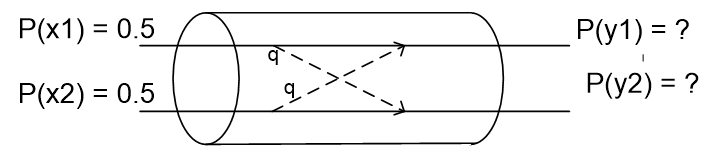
\includegraphics[width=.8\linewidth]{./02-kanalcodierung/fs2015}
    \vspace{-8pt}
\end{center}

Die Kanalmatrix ist gegeben mit:

$P(X|Y) = \begin{matrix}
    0.9 & 0.1\\
    0.2 & 0.8\\
\end{matrix}$

Ermitteln sie die Entropie am Kanaleingang H(x) und am Kanalausgang H(y). Ist der Kanal fehlerfrei?\\
$p(y_1)=0.5*0.9+0.5*0.2=0.55$\\
$p(y_2)=0.5*0.1+0.5*0.8=0.45$\\

$H(X)=-\sum_{i=1}^3p(x_i)*ld(p(x_i))$\\
$=-(0.5*ld(0.5)+0.5*ld(0.5))$\\
$=1$\\

$H(Y)=-\sum_{i=1}^3p(y_i)*ld(p(y_i))$\\
$=-(0.55*ld(0.55)+0.45*ld(0.45))$\\
$=0.99$\\

Der Kanal ist nicht fehlerfrei!

\subsection{Transinformation}
\subsubsection{Prüfung FS2009}
Sie messen einen binären Kanal aus und erhalten folgende Ergebnisse:\\

\begin{center}
    \centering
    \begin{tabular}{l | l | l}
        \bfseries{Zeichen} & \bfseries{gesendet}& \bfseries{Korrekt Empfangen}\\ \hline
        1 & 1000 & 980\\ 
        0 & 1000 & 650
    \end{tabular}
\end{center}

\paragraph{Geben Sie die Kanalmatrix an}\mbox{}\\

$\begin{bmatrix}
    0.98 & 0.02\\
    0.35 & 0.65\\
\end{bmatrix}$

Sie haben ebenfalls herausgefunden, dass die Auftrittswahrscheinlichkeiten der 2 Zeichen wie folgt ist:
\begin{itemize}
    \item Auftrittswahrscheinlichkeit für eine 1: P(1) = 0.7
    \item Auftrittswahrscheinlichkeit für eine 0: P(0) = 0.3
\end{itemize}

\paragraph{Berechnen Sie die Entropie für den Kanaleingang und den Kanalausgang}\mbox{}\\
$y_0=0.7*0.98+0.3*0.35=0.791$\\
$y_1=0.7*0.02+0.3*0.65=0.209$\\

$H(X)=-\sum_{i=1}^mp(x_i)*ld(p(x_i))$\\
Eingang: $H(X)=-(0.7*ld(0.7)+0.3*ld(0.3))=0.8813$\\
Ausgang: $H(Y)=-(0.791*ld(0.791)+0.209*ld(0.209))=0.7395$

\paragraph{Wie gross ist die Transinformation}\mbox{}\\
\begin{center}
    \vspace{-8pt}
    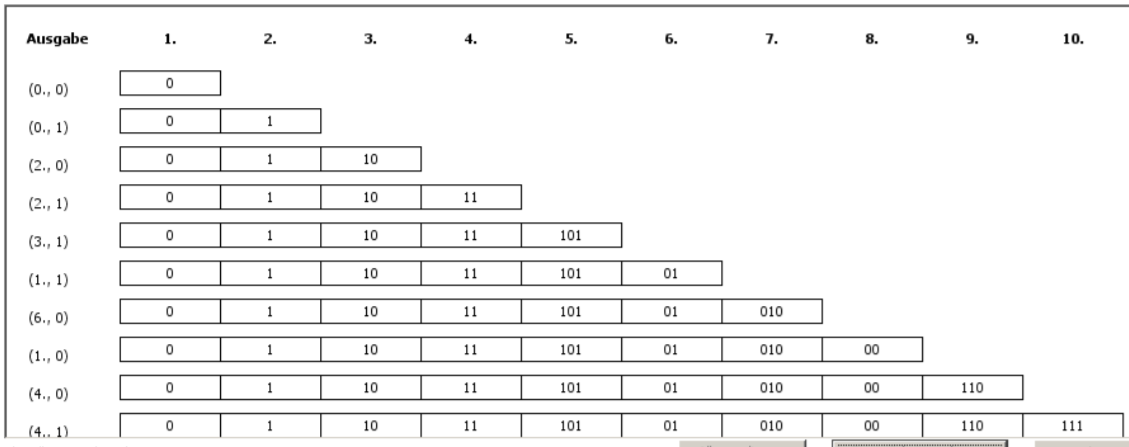
\includegraphics[width=.8\linewidth]{./02-kanalcodierung/fs2009}
    \vspace{-8pt}
\end{center}



